\documentclass[twocolumn, 12pt,letterpaper,english,bibliography=totocnumbered, abstract=on]{scrartcl}

\usepackage{indentfirst}
\usepackage[titletoc]{appendix}
%\usepackage{fullpage}
%\usepackage{subfiles}
\usepackage[T1]{fontenc}
\usepackage[latin9]{inputenc}
\usepackage{color}
\usepackage{babel}
\usepackage{verbatim}
\usepackage[unicode=true,pdfusetitle,
bookmarks=true,bookmarksnumbered=false,bookmarksopen=false,
breaklinks=true,pdfborder={0 0 0},pdfborderstyle={},backref=false,colorlinks=true]
{hyperref}
\hypersetup{linkcolor=blue,citecolor=blue,urlcolor=blue}

\usepackage{booktabs}
\usepackage{multirow}
\usepackage{adjustbox}
\usepackage{threeparttable}
\usepackage[table]{xcolor}
\usepackage{csquotes}
\usepackage{soul} % for hiliting text: \hl

\usepackage[backend=biber, style=authoryear, maxbibnames=99, dashed=false]{biblatex}
\setlength\bibitemsep{2\itemsep}
\addbibresource{mybib.bib}
%\addbibresource{CRB.bib}

\usepackage{pdfpages}
\usepackage{float} % Allows use of H to place floats

\usepackage{pgfgantt}

\usepackage{framed}

\usepackage[at]{easylist}

% Prevent page breaks within paragraphs
% https://tex.stackexchange.com/questions/21983/how-to-avoid-page-breaks-inside-paragraphs
\widowpenalties 1 10000

\begin{document}

%\titlehead{Work Plan: USDA Forest Service FY2020}

\title{DRAFT: Rethinking OrNV Bioassays}

\author{Aubrey Moore}

%\date{May 5, 2020\\Revised May 4, 2021}

\maketitle
%\footnote{\url{https://github.com/aubreymoore/2020-FS-CRB-biocontrol-project/blob/master/combined-proposal.pdf}}
%\newpage
\tableofcontents

%\pagebreak

\section{Introduction}

Bioassays designed to select isolates of OrNV as biocontrol agent candidates typically measuring differences in survival between beetles treated with one or more dosage levels and a an untreated experimental control group. However, the literature indicates that successful biocontrol of CRB by OrNV is caused by sublethal effects in addition to decreased survival. These include reduction in feeding rate, reproduction rate and flight activity \parencite{zelazny1977,prasad2008}. Theoretically, significant reduction in damage and population density can occur without any direct mortality from OrNV infection. It has been suggested that OrNV isolates which cause low mortality or even no mortality may be better biocontrol agent candidates than those which cause high mortality because they are better virus vectors.

Here I present a bioassay design to measure lethal and sublethal effects of OrNV. This idea was developed by myself and Mayuho Yamauchi, a PhD candidate working with Madoka Nakai at the Tokyo University of Agriculture and Technology. Mayuho Yamauchi visited my lab at the University of Guam during February and March 2022 and set up a bioassay to test an OrNV isolate from Palau using CRB adults from which were collected from pheromone traps on Guam. Some of our ideas were tested in this experiment.

The essential plan is to test groups of beetles kept in microcosms which mimic natural breeding sites (Fig. \ref{fig:setup}). Each microcosm consists of a one gallon paint can which is partially filled with moist cocopeat and supported a few inches above of a large garbage container with a top made from aluminum window screen. A bright white lighting fixture attached to a timer switch set for a 12 hour light-dark cycle is hung a few feet above the microcosms. At the start of a biossay a mixed-sex population of 20 to 30 individually numbered beetles is placed in the moist cocopeat within the paint bucket.  

\begin{figure}
	\centering
	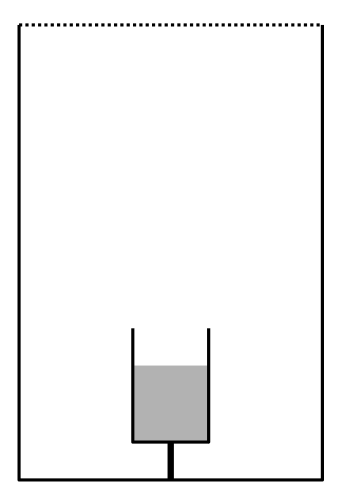
\includegraphics[width=0.7\linewidth]{images/setup.png}
	\caption{A microcosm for CRB bioassays}
	\label{fig:setup}
\end{figure}

\section{Protocol Prior to Start of Experiment}

\subsection{Test insects}

Ideally, test insects should come from a lab rearing colony which is free from pathogens and age of beetles is known. We are attempting to establish a lab colony on Guam but we are having technical difficulties and are not yet producing adults. For bioassays, we currently rely on adults collected from pheromone traps. The problem with these beetles is that individuals may be infected with \textit{Metarhizium majus} (released as a biocontrol agent on Guam), dying from exhaustion after struggling to escape entrapment, or dying from old age. Note that OrNV has not been detected in the Guam population.

We have developed a procedure to ensure the health of CRB used in our bioassays:
\begin{enumerate}
	\item We collect beetles from pheromone traps within 3 days after capture. Each beetle is placed into a Mason jar half filled with moist cocopeat in the field.  
	\item Upon return to our lab, each beetle is fed a 5mm thick banana slice and is fed similarly once a week thereafter.
	\item Beetles are quarantined in solitary confinement for at least 4 weeks prior to being selected as test insects.
\end{enumerate}

\subsection{Marking beetles}

We mark test beetles with unique identifiers so that we can maintain individual records for them using a laser engraving machine to etch serial numbers on elytra. (Previous attempts to mark beetles by hand or by using glue-on tags failed.)

While marking beetles, a table should be established with the following data: beetle id, date, sex, mass (mg), elytron length (mm) and elytron width (mm). See \cite{vandermeer1975} for elytral measurements.

\section{Protocol During Experiment} 

\subsection{Dosing}

Dosing method to be determined. Several methods are available including injection into haemocoel and  diet inclusion. \cite{zelazny1977} dosed adults by letting them swim for 10 min in a 10\% suspension of ground up, freshly virus-killed larvae.  

\subsection{Feeding}

While in quarantine beetles are fed weekly by adding a 5 mm thick slice of fresh banana to the surface of the moist cocopeat in each Mason jar in which beetles are confined.

During the bioassay, beetles are fed after each flying event. See \ref{daily activities}. 

\subsection{Observations}

Beetles become active shortly after the start of the scotophase. Some of these will fly out of the paint can and these will found at the bottom of the garbage container when checked during the following morning.

\subsubsection{Daily activities}
\label{daily activities}

\begin{enumerate}
	\item for each microcosm:
	\begin{enumerate}
        \item collect dead beetles on or near the surface of the cocopeat. Place dead beetles in individual pottles and place in freezer.
        \item check the bottom of the garbage container for beetles which few	
        \item for each beetle which flew:
        \begin{enumerate}
            \item weigh the beetle
            \item place the beetle in a Mason jar half filled with moist cocopeat
            \item place a 5 mm thick fresh banana slice on the surface of the cocopeat
            \item wait 24 h
            \item weigh the beetle again
            \item place the beetle back in its microcosm
        \end{enumerate}
    \end{enumerate}	   
\end{enumerate}

\subsubsection{Weekly activities}

\begin{enumerate}	
    \item for each microcosm:
    \begin{enumerate}
        \item remove all beetles from cocopeat. Place any dead beetles in individual pottles and place in freezer.
        \item weigh each live beetle
		\item transfer cocopeat from the microcosm into Mason jars and label these with treatment and current date. These jars will be examined in 3 weeks to count larvae. The 3 week delay will ensure that all viable eggs hatch, allowing calculation of reproductive rate per female.
		\item Half fill the microcosm paint bucket with fresh damp cocopeat and reintroduce beetles.
    \end{enumerate} 
\end{enumerate}

\pagebreak
\printbibliography

\end{document}
